%  LaTeX support: latex@mdpi.com 
%  For support, please attach all files needed for compiling as well as the log file, and specify your operating system, LaTeX version, and LaTeX editor.

%=================================================================
\documentclass[journal,article,submit,pdftex,moreauthors]{Definitions/mdpi} 
%\documentclass[preprints,article,submit,pdftex,moreauthors]{Definitions/mdpi} 
% For posting an early version of this manuscript as a preprint, you may use "preprints" as the journal. Changing "submit" to "accept" before posting will remove line numbers.

% Below journals will use APA reference format:
% admsci, aieduc, behavsci, businesses, econometrics, economies, education, ejihpe, famsci, games, humans, ijcs, ijfs, journalmedia, jrfm, languages, psycholint, publications, tourismhosp, youth

% Below journals will use Chicago reference format:
% arts, genealogy, histories, humanities, jintelligence, laws, literature, religions, risks, socsci

%--------------------
% Class Options:
%--------------------
%----------
% journal
%----------
% Choose between the following MDPI journals:
% accountaudit, acoustics, actuators, addictions, adhesives, admsci, adolescents, aerobiology, aerospace, agriculture, agriengineering, agrochemicals, agronomy, ai, air, algorithms, allergies, alloys, amh, analytica, analytics, anatomia, anesthres, animals, antibiotics, antibodies, antioxidants, applbiosci, appliedchem, appliedmath, appliedphys, applmech, applmicrobiol, applnano, applsci, aquacj, architecture, arm, arthropoda, arts, asc, asi, astronomy, atmosphere, atoms, audiolres, automation, axioms, bacteria, batteries, bdcc, behavsci, beverages, biochem, bioengineering, biologics, biology, biomass, biomechanics, biomed, biomedicines, biomedinformatics, biomimetics, biomolecules, biophysica, biosensors, biosphere, biotech, birds, blockchains, bloods, blsf, brainsci, breath, buildings, businesses, cancers, carbon, cardiogenetics, catalysts, cells, ceramics, challenges, chemengineering, chemistry, chemosensors, chemproc, children, chips, cimb, civileng, cleantechnol, climate, clinbioenerg, clinpract, clockssleep, cmd, cmtr, coasts, coatings, colloids, colorants, commodities, complications, compounds, computation, computers, condensedmatter, conservation, constrmater, cosmetics, covid, crops, cryo, cryptography, crystals, csmf, ctn, curroncol, cyber, dairy, data, ddc, dentistry, dermato, dermatopathology, designs, devices, diabetology, diagnostics, dietetics, digital, disabilities, diseases, diversity, dna, drones, dynamics, earth, ebj, ecm, ecologies, econometrics, economies, education, eesp, ejihpe, electricity, electrochem, electronicmat, electronics, encyclopedia, endocrines, energies, eng, engproc, ent, entomology, entropy, environments, epidemiologia, epigenomes, esa, est, famsci, fermentation, fibers, fintech, fire, fishes, fluids, foods, forecasting, forensicsci, forests, fossstud, foundations, fractalfract, fuels, future, futureinternet, futureparasites, futurepharmacol, futurephys, futuretransp, galaxies, games, gases, gastroent, gastrointestdisord, gastronomy, gels, genealogy, genes, geographies, geohazards, geomatics, geometry, geosciences, geotechnics, geriatrics, glacies, grasses, greenhealth, gucdd, hardware, hazardousmatters, healthcare, hearts, hemato, hematolrep, heritage, higheredu, highthroughput, histories, horticulturae, hospitals, humanities, humans, hydrobiology, hydrogen, hydrology, hygiene, idr, iic, ijerph, ijfs, ijgi, ijmd, ijms, ijns, ijpb, ijt, ijtm, ijtpp, ime, immuno, informatics, information, infrastructures, inorganics, insects, instruments, inventions, iot, j, jal, jcdd, jcm, jcp, jcs, jcto, jdad, jdb, jeta, jfb, jfmk, jimaging, jintelligence, jlpea, jmahp, jmmp, jmms, jmp, jmse, jne, jnt, jof, joitmc, joma, jop, jor, journalmedia, jox, jpbi, jpm, jrfm, jsan, jtaer, jvd, jzbg, kidney, kidneydial, kinasesphosphatases, knowledge, labmed, laboratories, land, languages, laws, life, lights, limnolrev, lipidology, liquids, literature, livers, logics, logistics, lubricants, lymphatics, machines, macromol, magnetism, magnetochemistry, make, marinedrugs, materials, materproc, mathematics, mca, measurements, medicina, medicines, medsci, membranes, merits, metabolites, metals, meteorology, methane, metrics, metrology, micro, microarrays, microbiolres, microelectronics, micromachines, microorganisms, microplastics, microwave, minerals, mining, mmphys, modelling, molbank, molecules, mps, msf, mti, multimedia, muscles, nanoenergyadv, nanomanufacturing, nanomaterials, ncrna, ndt, network, neuroglia, neurolint, neurosci, nitrogen, notspecified, nursrep, nutraceuticals, nutrients, obesities, oceans, ohbm, onco, oncopathology, optics, oral, organics, organoids, osteology, oxygen, parasites, parasitologia, particles, pathogens, pathophysiology, pediatrrep, pets, pharmaceuticals, pharmaceutics, pharmacoepidemiology, pharmacy, philosophies, photochem, photonics, phycology, physchem, physics, physiologia, plants, plasma, platforms, pollutants, polymers, polysaccharides, populations, poultry, powders, preprints, proceedings, processes, prosthesis, proteomes, psf, psych, psychiatryint, psychoactives, psycholint, publications, purification, quantumrep, quaternary, qubs, radiation, reactions, realestate, receptors, recycling, regeneration, religions, remotesensing, reports, reprodmed, resources, rheumato, risks, robotics, rsee, ruminants, safety, sci, scipharm, sclerosis, seeds, sensors, separations, sexes, signals, sinusitis, siuj, skins, smartcities, sna, societies, socsci, software, soilsystems, solar, solids, spectroscj, sports, standards, stats, std, stresses, surfaces, surgeries, suschem, sustainability, symmetry, synbio, systems, tae, targets, taxonomy, technologies, telecom, test, textiles, thalassrep, therapeutics, thermo, timespace, tomography, tourismhosp, toxics, toxins, transplantology, transportation, traumacare, traumas, tropicalmed, universe, urbansci, uro, vaccines, vehicles, venereology, vetsci, vibration, virtualworlds, viruses, vision, waste, water, wem, wevj, wild, wind, women, world, youth, zoonoticdis

%---------
% article
%---------
% The default type of manuscript is "article", but can be replaced by: 
% abstract, addendum, article, benchmark, book, bookreview, briefcommunication, briefreport, casereport, changes, clinicopathologicalchallenge, comment, commentary, communication, conceptpaper, conferenceproceedings, correction, conferencereport, creative, datadescriptor, discussion, entry, expressionofconcern, extendedabstract, editorial, essay, erratum, fieldguide, hypothesis, interestingimages, letter, meetingreport, monograph, newbookreceived, obituary, opinion, proceedingpaper, projectreport, reply, retraction, review, perspective, protocol, shortnote, studyprotocol, supfile, systematicreview, technicalnote, viewpoint, guidelines, registeredreport, tutorial,  giantsinurology, urologyaroundtheworld
% supfile = supplementary materials

%----------
% submit
%----------
% The class option "submit" will be changed to "accept" by the Editorial Office when the paper is accepted. This will only make changes to the frontpage (e.g., the logo of the journal will get visible), the headings, and the copyright information. Also, line numbering will be removed. Journal info and pagination for accepted papers will also be assigned by the Editorial Office.

%------------------
% moreauthors
%------------------
% If there is only one author the class option oneauthor should be used. Otherwise use the class option moreauthors.

%---------
% pdftex
%---------
% The option pdftex is for use with pdfLaTeX. Remove "pdftex" for (1) compiling with LaTeX & dvi2pdf (if eps figures are used) or for (2) compiling with XeLaTeX.

%=================================================================
% MDPI internal commands - do not modify
\firstpage{1} 
\makeatletter 
\setcounter{page}{\@firstpage} 
\makeatother
\pubvolume{1}
\issuenum{1}
\articlenumber{0}
\pubyear{2025}
\copyrightyear{2025}
%\externaleditor{Firstname Lastname} % More than 1 editor, please add `` and '' before the last editor name
\datereceived{ } 
\daterevised{ } % Comment out if no revised date
\dateaccepted{ } 
\datepublished{ } 
%\datecorrected{} % For corrected papers: "Corrected: XXX" date in the original paper.
%\dateretracted{} % For retracted papers: "Retracted: XXX" date in the original paper.
\hreflink{https://doi.org/} % If needed use \linebreak
%\doinum{}
%\pdfoutput=1 % Uncommented for upload to arXiv.org
%\CorrStatement{yes}  % For updates
%\longauthorlist{yes} % For many authors that exceed the left citation part

%=================================================================
% Add packages and commands here. The following packages are loaded in our class file: fontenc, inputenc, calc, indentfirst, fancyhdr, graphicx, epstopdf, lastpage, ifthen, float, amsmath, amssymb, lineno, setspace, enumitem, mathpazo, booktabs, titlesec, etoolbox, tabto, xcolor, colortbl, soul, multirow, microtype, tikz, totcount, changepage, attrib, upgreek, array, tabularx, pbox, ragged2e, tocloft, marginnote, marginfix, enotez, amsthm, natbib, hyperref, cleveref, scrextend, url, geometry, newfloat, caption, draftwatermark, seqsplit
% cleveref: load \crefname definitions after \begin{document}

%=================================================================
% Please use the following mathematics environments: Theorem, Lemma, Corollary, Proposition, Characterization, Property, Problem, Example, ExamplesandDefinitions, Hypothesis, Remark, Definition, Notation, Assumption
%% For proofs, please use the proof environment (the amsthm package is loaded by the MDPI class).

%=================================================================
% Full title of the paper (Capitalized)
\Title{Design and Implementation of a UART Module on FPGA Using RTL for Cryptographic Encryption and Decryption Techniques}

% MDPI internal command: Title for citation in the left column
\TitleCitation{Title}

% Author Orchid ID: enter ID or remove command
\newcommand{\orcidauthorA}{0000-0000-0000-000X} % Add \orcidA{} behind the author's name
%\newcommand{\orcidauthorB}{0000-0000-0000-000X} % Add \orcidB{} behind the author's name

% Authors, for the paper (add full first names)
\Author{Christian-Antonio Colin-Cejudo$^{1,\dagger,\ddagger}$\orcidA{}, Gonzalo-Issac Duchén-Sánchez $^{2,\ddagger}$ and Firstname Lastname $^{2,}$*}

%\longauthorlist{yes}

% MDPI internal command: Authors, for metadata in PDF
\AuthorNames{Firstname Lastname, Firstname Lastname and Firstname Lastname}

% MDPI internal command: Authors, for citation in the left column, only choose below one of them according to the journal style
% If this is a Chicago style journal 
% (arts, genealogy, histories, humanities, jintelligence, laws, literature, religions, risks, socsci): 
% Lastname, Firstname, Firstname Lastname, and Firstname Lastname.

% If this is a APA style journal 
% (admsci, behavsci, businesses, econometrics, economies, education, ejihpe, games, humans, ijfs, journalmedia, jrfm, languages, psycholint, publications, tourismhosp, youth): 
% Lastname, F., Lastname, F., \& Lastname, F.

% If this is a ACS style journal (Except for the above Chicago and APA journals, all others are in the ACS format): 
% Lastname, F.; Lastname, F.; Lastname, F.
\isAPAStyle{%
       \AuthorCitation{Lastname, F., Lastname, F., \& Lastname, F.}
         }{%
        \isChicagoStyle{%
        \AuthorCitation{Lastname, Firstname, Firstname Lastname, and Firstname Lastname.}
        }{
        \AuthorCitation{Lastname, F.; Lastname, F.; Lastname, F.}
        }
}

% Affiliations / Addresses (Add [1] after \address if there is only one affiliation.)
\address{%
$^{1}$ \quad Affiliation 1; christian.upiita@gmai.com\\
$^{2}$ \quad Affiliation 2; gduchen@ieee.org}

% Contact information of the corresponding author
\corres{Correspondence: e-mail@e-mail.com; Tel.: (optional; include country code; if there are multiple corresponding authors, add author initials) +xx-xxxx-xxx-xxxx (F.L.)}

% Current address and/or shared authorship
\firstnote{Current address: Affiliation.}  % Current address should not be the same as any items in the Affiliation section.
\secondnote{These authors contributed equally to this work.}
% The commands \thirdnote{} till \eighthnote{} are available for further notes

%\simplesumm{} % Simple summary

%\conference{} % An extended version of a conference paper

% Abstract (Do not insert blank lines, i.e. \\) 
\abstract{The increasing demand for robust and efficient information security has led to the growing adoption of specialized hardware for cryptographic operations. In response to the rise in cyber threats and the need to process large volumes of data in real time, hardware-based cryptographic solutions offer significant advantages in terms of performance, resistance to attacks, and secure storage of cryptographic keys. This thesis presents the implementation of a secure communication system using the UART (Universal Asynchronous Receiver-Transmitter) protocol as the foundation for a Register Transfer Level (RTL) design on an FPGA platform. The base protocol was modified to introduce an additional hardware-level security layer. Furthermore, cryptographic techniques—specifically encryption and decryption—were integrated into the design to enhance data protection and integrity during transmission. The results demonstrate the feasibility of embedding cryptographic mechanisms directly into communication hardware, providing a scalable and efficient solution for secure embedded systems.}

% Keywords
\keyword{Cryptographic hardware; Information security; Encryption, Decryption; Cryptographic keys; Digital signatures; Authentication; Cyber threats; Data processing; Communication protocols; UART (Universal Asynchronous Receiver-Transmitter); FPGA (Field-Programmable Gate Array); RTL design (Register Transfer Level); Hardware security layer; Cryptographic techniques; Critical infrastructure.} 

% The fields PACS, MSC, and JEL may be left empty or commented out if not applicable
%\PACS{J0101}
%\MSC{}
%\JEL{}

%%%%%%%%%%%%%%%%%%%%%%%%%%%%%%%%%%%%%%%%%%
% Only for the journal Diversity
%\LSID{\url{http://}}

%%%%%%%%%%%%%%%%%%%%%%%%%%%%%%%%%%%%%%%%%%
% Only for the journal Applied Sciences
%\featuredapplication{Authors are encouraged to provide a concise description of the specific application or a potential application of the work. This section is not mandatory.}
%%%%%%%%%%%%%%%%%%%%%%%%%%%%%%%%%%%%%%%%%%

%%%%%%%%%%%%%%%%%%%%%%%%%%%%%%%%%%%%%%%%%%
% Only for the journal Data
%\dataset{DOI number or link to the deposited data set if the data set is published separately. If the data set shall be published as a supplement to this paper, this field will be filled by the journal editors. In this case, please submit the data set as a supplement.}
%\datasetlicense{License under which the data set is made available (CC0, CC-BY, CC-BY-SA, CC-BY-NC, etc.)}

%%%%%%%%%%%%%%%%%%%%%%%%%%%%%%%%%%%%%%%%%%
% Only for the journal BioTech, Fishes, Neuroimaging and Toxins
%\keycontribution{The breakthroughs or highlights of the manuscript. Authors can write one or two sentences to describe the most important part of the paper.}

%%%%%%%%%%%%%%%%%%%%%%%%%%%%%%%%%%%%%%%%%%
% Only for the journal Encyclopedia
%\encyclopediadef{For entry manuscripts only: please provide a brief overview of the entry title instead of an abstract.}

%%%%%%%%%%%%%%%%%%%%%%%%%%%%%%%%%%%%%%%%%%
% Only for the journal Advances in Respiratory Medicine, Future, Sensors and Smart Cities
%\addhighlights{yes}
%\renewcommand{\addhighlights}{%
%
%\noindent This is an obligatory section in ``Advances in Respiratory Medicine'', ``Future'', ``Sensors'' and ``Smart Cities”, whose goal is to increase the discoverability and readability of the article via search engines and other scholars. Highlights should not be a copy of the abstract, but a simple text allowing the reader to quickly and simplified find out what the article is about and what can be cited from it. Each of these parts should be devoted up to 2~bullet points.\vspace{3pt}\\
%\textbf{What are the main findings?}
% \begin{itemize}[labelsep=2.5mm,topsep=-3pt]
% \item First bullet.
% \item Second bullet.
% \end{itemize}\vspace{3pt}
%\textbf{What is the implication of the main finding?}
% \begin{itemize}[labelsep=2.5mm,topsep=-3pt]
% \item First bullet.
% \item Second bullet.
% \end{itemize}
%}

%%%%%%%%%%%%%%%%%%%%%%%%%%%%%%%%%%%%%%%%%%
\begin{document}

%%%%%%%%%%%%%%%%%%%%%%%%%%%%%%%%%%%%%%%%%%
\setcounter{section}{0} %% Remove this when starting to work on the template.
%\section{How to Use this Template}


% The order of the section titles is different for some journals. Please refer to the "Instructions for Authors” on the journal homepage.

\section{Introduction}

Currently, information security has become a fundamental pillar for the development of reliable digital systems. The increasing sophistication of cyber threats, combined with the exponential growth in data generation and transmission, demands increasingly robust and efficient solutions. In this context, the use of specialized hardware for cryptographic operations has emerged as an effective alternative to the limitations of software-only cryptographic processing.

Cryptographic hardware offers significant advantages, such as higher performance, lower latency, reduced energy consumption, and greater resistance to both physical and logical attacks. These characteristics make it an ideal solution for embedded systems, IoT devices, industrial applications, and environments where security and operational efficiency are top priorities.

Field Programmable Gate Arrays (FPGAs) have become one of the most versatile technologies for electronic system design. These devices provide a cost-effective solution, especially for low-volume production, since the initial cost of prototyping is considerably lower compared to Application-Specific Integrated Circuits (ASICs). Moreover, a key advantage is their reconfigurability during operation, which allows a single device to perform multiple predefined functions, thereby optimizing space and reducing costs.

Today, electronic systems are present in almost every aspect of daily life, from consumer products to industrial control systems, automotive applications, security, and beyond. The current trend in electronic design is characterized by the increasing complexity of components, which demands solutions that are user-friendly, versatile, low-power, and quick to market. Modern integrated circuit technology makes it possible to integrate these complex systems into highly compact dimensions, referred to as embedded systems or Systems on Chip (SoC). These systems, designed to fulfill specific functions, combine hardware and software tailored for each task. In this context, FPGAs, thanks to their reconfigurability, are valuable tools for developing prototypes or small-scale series at affordable costs.

Among the most widely used communication protocols in embedded systems is the Universal Asynchronous Receiver-Transmitter (UART), due to its simplicity, low implementation cost, and broad compatibility. However, this protocol lacks native security mechanisms, making it vulnerable to interception, manipulation, and unauthorized access.

This thesis proposes the design and implementation of a cryptographic security layer on top of the UART protocol, using a Register Transfer Level (RTL) approach on an FPGA platform. The implementation leverages a Hardware Description Language (HDL) to model and design digital circuits. The modification of the protocol not only ensures secure data transmission but also integrates encryption and decryption techniques directly into hardware. This solution aims to demonstrate the feasibility of incorporating efficient cryptographic security into embedded communication systems without compromising performance or scalability. 

%%%%%%%%%%%%%%%%%%%%%%%%%%%%%%%%%%%%%%%%%%
\section{Materials and Methods}
To properly contextualize the present thesis, it is necessary to address the origins of the standard cryptographic algorithm Caesar, as well as its evolution and applications over time. Likewise, the conditions under which information security services and mechanisms emerged will be explored, along with the ways in which they have been implemented across different environments. This analysis allows for the delineation of the problem that this research seeks to address through the proposed hardware-based implementation. Consequently, a review of the state of the art in the field is carried out, with particular emphasis on embedded systems that incorporate security mechanisms.

This review seeks to establish the foundations underlying the design of cryptographic solutions on reconfigurable platforms such as FPGAs, highlighting their relevance in scenarios where information protection is critical. This theoretical framework provides the basis for the methodological and experimental development presented in the following chapters.

\subsection{Classical Cryptography Fundamentals}
Cryptography is the science and art of protecting information through techniques that transform readable data (plaintext) into unintelligible data (ciphertext), so that only authorized individuals can access its content (Stallings, 2017). Throughout history, cryptography has evolved from simple substitution and transposition methods to complex algorithms based on mathematical theory, modern algebra, and number theory.

Although classical methods are now considered insecure against modern attacks, they provide a foundation for understanding fundamental concepts such as key usage, symmetric encryption, and cryptanalysis. One of the most representative algorithms of classical cryptography is the Caesar cipher, also known as the shift cipher.

\subsection{The Caesar Cipher: Historical Background}
The Caesar cipher is named after Julius Caesar, who used it to encrypt military communications. Historical records indicate that Caesar applied a shift of three positions to encode his messages (Kahn, 1996). While its simplicity renders it trivial by modern standards, at the time it provided a basic level of protection against untrained or illiterate readers.

This cipher is classified as a monoalphabetic substitution cipher, in which each letter of the alphabet is systematically replaced by another according to a fixed shift key.
\subsection{Operation of the Algorithm}
From a mathematical perspective, the Caesar cipher can be represented by the following function:
\centerline{\(C(x) = ( x + k ) mod n \)}

Where:

\begin{itemize}
\item $C(x)$ is the encrypted character.
\item $x$ is the index of the character in the alphabet $A = 0, B = 1, \dots, Z = 25$.
\item $k$ is the shift key.
\item $n$ is the total number of characters in the alphabet, usually $n = 26$ for the Latin alphabet.
\end{itemize}

Decryption consists of applying the inverse operation:

\centerline{$P(x) = ( x - k ) \bmod n $}

For example, if the word \textbf{\textit{“HOLA”}} is encrypted with a shift of $k = 3$, the result is \textbf{\textit{“KROD”}}. To decrypt, the inverse shift is applied.

\subsection{Security and Vulnerabilities}

The Caesar cipher is vulnerable to several types of cryptographic attacks:

\begin{itemize}
\item \textbf{Brute-force attack:} Since there are only 25 possible keys (excluding the null shift), an attacker can test all combinations in a short time.
\item \textbf{Frequency analysis:} Each language has a characteristic letter distribution. In Spanish, the letters E'', A'', and ''O'' are the most common. If a sufficiently long text is encrypted, these frequencies are preserved, allowing the shift used to be identified.
\end{itemize}

These weaknesses make it unsuitable for any modern application requiring real confidentiality, but it remains useful as a development and educational tool.

\subsection{Usefulness in Cryptographic System Design}

Despite its limitations, the Caesar cipher is frequently used in the design of hardware/software cryptographic systems for educational and experimental purposes. Its simple structure makes it an ideal choice for:

\begin{itemize}
\item Introducing sequential data processing techniques.
\item Implementing finite state machines for encoding and decoding.
\item Evaluating logical resource usage and propagation delays on platforms such as FPGAs.
\item Comparing the behavior of more complex ciphers with respect to basic algorithms in low-level environments (VHDL, Verilog).
\end{itemize}

In digital design projects with RTL (Register Transfer Level) architecture, the Caesar cipher is used as a case study to optimize modular shift operations, ASCII character encoding, and key generation.



\subsection{Background on SystemVerilog}

\subsection{Evolution of Digital Design and the Emergence of SystemVerilog}

The development of digital design has undergone significant transformations since its inception, beginning with physical prototyping using breadboards and evolving to sophisticated computer-aided simulation and modeling platforms. CAD (Computer-Aided Design) tools allowed for more precise and efficient simulation of electronic circuits, although their initial use required overcoming certain technical complexity barriers.

These tools facilitated the implementation of electrical schematics and enabled the definition of input signals consistent with system logic, producing outputs that were easily interpretable. Simulators such as SPICE became benchmarks in both academic and industrial settings by providing accurate modeling of electrical behavior. Once results were validated, the physical circuit design was carried out using specialized printed circuit board (PCB) tools, such as the OrCAD environment, particularly its PCB Layout module.

During this stage, the Adaptable Computing Laboratory began implementing electronic neural circuit models using these platforms (Padrón, 1997). Later, as the complexity of neural network models increased, tools such as MATLAB and its graphical environment SIMULINK were incorporated, allowing a direct mathematical representation of dynamic systems. This evolution enabled more effective interpretation of results, both quantitatively and qualitatively (Padrón et al., 2000, pp. 338–349).

In parallel, the reconfigurable hardware industry, particularly through FPGA boards manufactured by Xilinx, allowed addressing specific problems via programmable interfaces. Each board is designed to offer flexibility to the user, who can program its components in hardware description languages such as Verilog or VHDL and integrate various interfaces depending on the physical or logical availability of the system. This versatility made development kits fundamental tools for designing custom solutions, especially in rapid prototyping and functional validation contexts.

As system-level design requirements grew and verification became a critical stage, SystemVerilog emerged as an extension and evolution of the Verilog language. SystemVerilog not only incorporated improvements in structural and behavioral hardware description but also integrated capabilities for functional verification, object-oriented programming, and complex system modeling. This evolution addressed the need to unify the design and verification flow under a single language, facilitating the implementation of advanced testbenches, reusable interfaces, and verification environments compatible with modern methodologies such as UVM (Universal Verification Methodology).

In this regard, the use of FPGA boards programmed with SystemVerilog allows combining the precision of RTL design with advanced verification capabilities, which is essential in development environments aiming to ensure functionality, performance, and reliability from the early stages of a project. The history and evolution of this language reflect a trend toward consolidating tools that integrate design, simulation, verification, and synthesis within a single development environment.

\textbf{Relevant chronology of SystemVerilog development:}
\begin{itemize}
\item 1984: The Verilog language is introduced as a hardware description tool by Gateway Design Automation, later acquired by Cadence (IEEE, 2008).
\item 1990s: Verilog becomes one of the main standards for digital design, widely used in the electronics industry.
\item 1999: Development of SystemVerilog begins as an extension of Verilog to address limitations in verification and modeling (Accellera Systems Initiative, 2002).
\item 2002: SystemVerilog is formally adopted by Accellera as a standard for design and verification.
\item 2005: SystemVerilog is standardized by IEEE as IEEE 1800-2005, consolidating its industrial use (IEEE, 2005).
\item 2012: The IEEE 1800-2012 revision is published, incorporating improvements in synthesis and verification.
\item 2017: The IEEE 1800-2017 revision is published, expanding features for complex system design and verification.
\end{itemize}

\subsection{Hardware Description Languages (HDL) and Their Application in Digital Design}

Hardware Description Languages (HDL) emerged in response to the need for digital designers to have formal tools that allow the specification, modeling, and verification of digital systems in a structured manner and at different levels of abstraction. These languages not only facilitate communication among designers but also enable smooth interaction between computer-aided design (CAD) tools and the digital models themselves (Terés et al., 1998).

HDL-based development environments integrate compilation, simulation, and synthesis tools, allowing the functional behavior of a design to be validated before its physical implementation. Today, the most widely used HDL languages are VHDL and Verilog, both standardized by the IEEE (Institute of Electrical and Electronics Engineers) and broadly adopted in the digital design industry.

\textbf{VHDL: Description, Application, and Structure}

VHDL (VHSIC Hardware Description Language) was originally developed to document and verify high-speed integrated circuits within the VHSIC program of the U.S. Department of Defense. Its syntax and semantics are based on the ADA programming language, providing a robust structure suitable for critical and real-time systems.

VHDL allows modeling a digital system at different levels of description: behavioral, register-transfer level (RTL), and structural logic level. This enables coverage of nearly the entire digital development cycle, from functional specifications to prototype generation, excluding only the physical layout.

The correct choice of abstraction level in the description depends on the design objective. For instance, if the goal is to generate a physical implementation using synthesis tools, the RTL level is preferred. In contrast, to validate the functionality of complex algorithms through simulation, the algorithmic level is more appropriate (Baena, 2010).


\subsection{Comparison between Hardware Description Languages and Software Development}

Since their inception, various computer-aided design (CAD) tools and environments have employed specific languages and formats to represent and manage the diverse elements involved in electronic design. Some of these languages consisted of explicit notations used by the designer to describe inputs to particular tools, while others corresponded to internal intermediate formats, optimized for automated processing within the CAD environment and generally hidden from the designer.

However, these descriptions were limited to the particular ecosystem of each tool, offering neither portability nor standardization. The emergence of Hardware Description Languages (HDL) represented a significant advance by introducing a higher degree of standardization and incorporating principles from software engineering into the specification and modeling of digital hardware.

From a syntactic perspective, HDLs share similarities with high-level programming languages (HLL), which facilitates their learning for engineers with prior software development experience. For example, Verilog shares many features with the C language, whereas VHDL inherits its structure and semantics from the ADA language. While these similarities can accelerate HDL adoption, they can also lead to conceptual errors if software-oriented strategies are applied in contexts where an accurate representation of the hardware's physical behavior is required.

It is essential that, when an HDL model is intended for synthesis and physical implementation (e.g., on FPGAs or ASICs), the designer adopts a hardware-oriented mindset, describing the logic using a structural or register-transfer level (RTL) approach rather than merely an algorithmic one. Conversely, employing software-like structures can be appropriate when the goal is solely functional simulation of the system, optimizing performance during verification and timing analysis stages.

In summary, HDLs are high-level formal languages specifically designed to represent electronic circuits at various levels of abstraction—from basic logic gates to complete digital systems—and allow flexible, structured, and precise hardware modeling, leveraging concepts from both electronic design and software development, as shown in Figure \ref{fig:imagen1}.

\begin{figure}[h!]
\centering
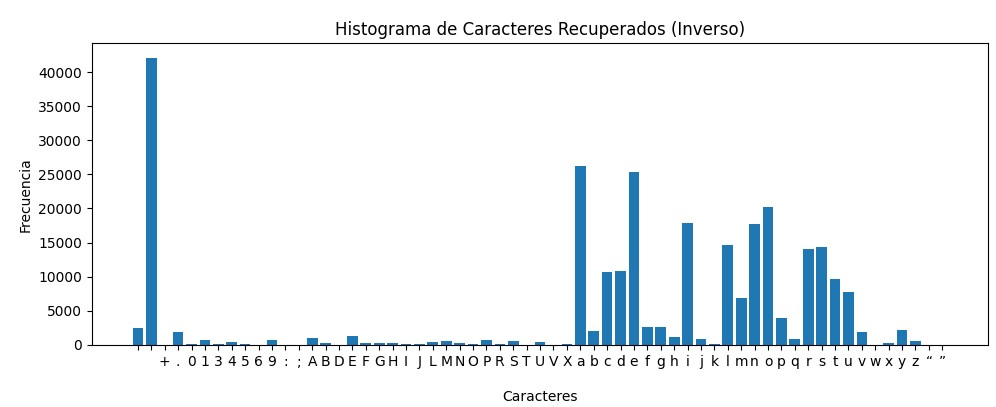
\includegraphics[width=0.5\textwidth, height=6cm]{imagenes/img1}
\caption{Abstraction/precision levels and VHDL modeling styles.}
\label{fig:imagen1}
\end{figure}

HDLs were initially developed to model the functional behavior of electronic components, enabling simulation prior to physical implementation. Nevertheless, they are also widely used for the structural description of digital circuits, facilitating subsequent synthesis and verification through validated simulation processes (Figure \ref{fig:imagen2}).

\begin{figure}[h!]
\centering
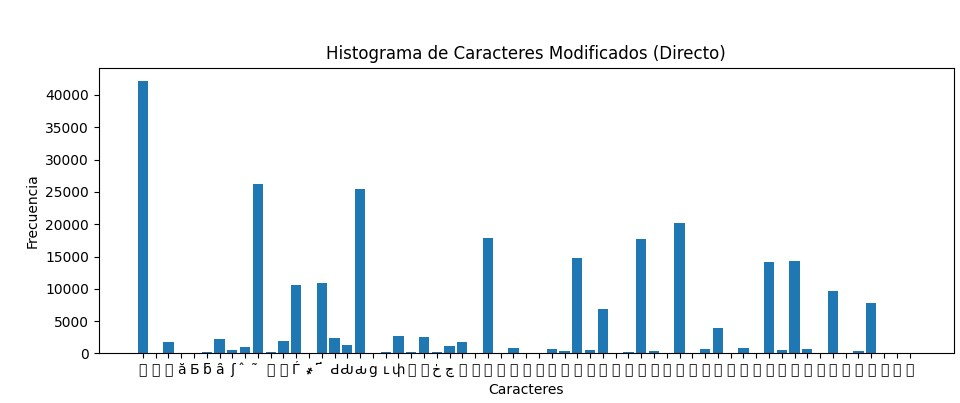
\includegraphics[width=0.7\textwidth, height=6cm]{imagenes/img2}
\caption{Software versus hardware development: (a) abstraction levels and high-level languages, and (b) basic top-down design scheme using HDL.}
\label{fig:imagen2}
\end{figure}

Building on the initial descriptions, top-down design approaches allow progressive synthesis processes that gradually lead to more detailed implementation levels, ultimately achieving a specific, technology-dependent physical description. Validation at each stage of the design is performed through functional simulations and analyses, enabling successive verification and correction iterations until the behavior conforms to the specified requirements (Figure \ref{fig:imagen2}(b)).


\section{Description of the Altera DE2-115 Development Board}

The Altera DE2-115 board, developed by Terasic Technologies, is a prototyping platform based on the Altera (now Intel) Cyclone IV EP4CE115F29C7N FPGA, designed for educational environments, research, and advanced digital system development. This board offers a versatile architecture that allows implementation ranging from basic logic designs to complex digital systems, including embedded systems, custom controllers, digital signal processing (DSP), and System-on-Chip (SoC) prototypes.

Key features include 114,480 logic elements (LEs), 3,888 Kbits of embedded RAM, and 528 general-purpose input/output (GPIO) pins, providing significant flexibility for interfacing with multiple peripheral devices. The board also includes external memory such as 128 MB SDRAM, 2 MB SRAM, and 2 MB NOR Flash, in addition to SD card support for external storage.

The DE2-115 incorporates essential interfaces for developing interactive systems, including USB ports, Gigabit Ethernet, VGA output, audio input/output, and a set of integrated user I/O devices such as switches, buttons, LEDs, and seven-segment displays. Additionally, it features a 50 MHz crystal oscillator and expansion connectors compatible with additional modules.

This platform is widely used in academic laboratories and applied research environments due to its compatibility with development tools such as Quartus Prime, facilitating the implementation of designs in HDL languages like VHDL and SystemVerilog. Its capability to perform simulation, verification, and synthesis of designs within a single tool makes it ideal for higher education projects in electronic engineering, mechatronics, and digital systems Figure \ref{fig:imagen3}.

\textbf{Highlighted Technical Specifications:}

\textbf{FPGA:} Altera Cyclone IV EP4CE115F29C7N with 114,480 logic elements (LEs)

\begin{itemize}
\item \textbf{Memory:}
\begin{itemize}
\item 2 MB SRAM
\item 128 MB SDRAM
\item 2 MB NOR Flash
\item SD card for external storage
\end{itemize}
\item \textbf{User Interfaces:}
\begin{itemize}
\item 18 switches and 18 push-buttons
\item 18 red LEDs and 9 green LEDs
\item 8 seven-segment displays
\end{itemize}
\item \textbf{Connectivity:}
\begin{itemize}
\item USB Type-A and Type-B ports
\item 10/100/1000 Mbps Ethernet port (Gigabit)
\item VGA input/output
\item 40-pin GPIO expansion connectors
\end{itemize}
\item \textbf{Audio and Video:}
\begin{itemize}
\item Audio input/output (3.5 mm jack)
\item VGA signal input (with ADC) and VGA output
\end{itemize}
\item \textbf{Clock:} 50 MHz crystal oscillator
\item \textbf{Programming and Debugging:} JTAG support, compatible with Quartus II
\end{itemize}

\begin{figure}[h!]
\centering
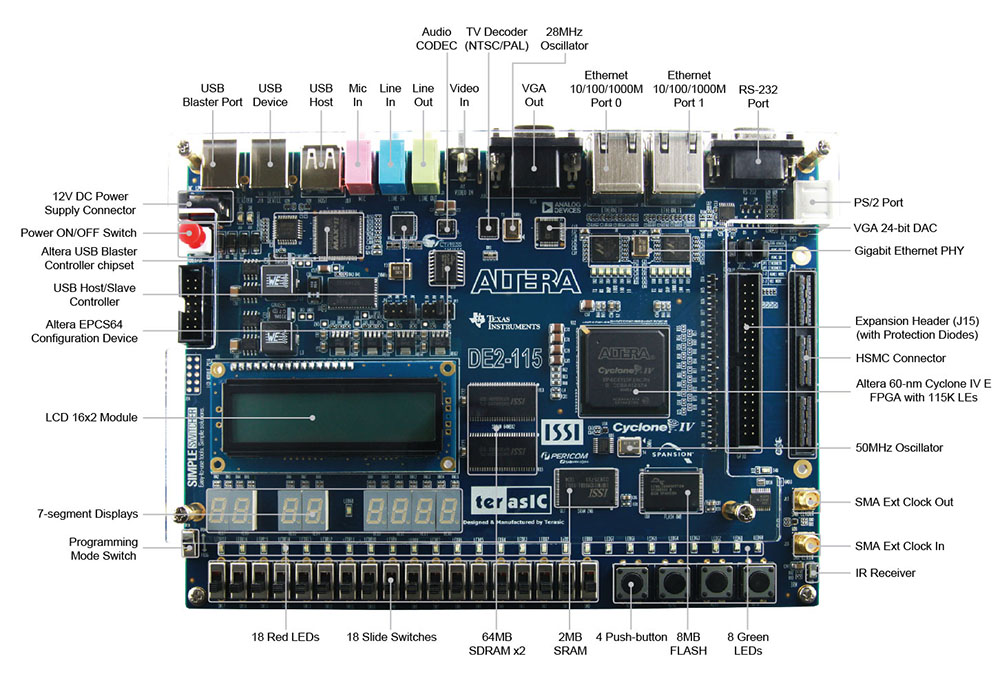
\includegraphics[width=1\textwidth, height=13cm]{imagenes/img3}
\caption{Altera DE2-115 Development Board.}
\label{fig:imagen3}
\end{figure}

\begin{quote}
This is an example of a quote.
\end{quote}

%%%%%%%%%%%%%%%%%%%%%%%%%%%%%%%%%%%%%%%%%%
\section{Results}



This section may be divided by subheadings. It should provide a concise and precise description of the experimental results, their interpretation as well as the experimental conclusions that can be drawn.
\subsection{Subsection}
\subsubsection{Subsubsection}

Bulleted lists look like this:
\begin{itemize}
\item	First bullet;
\item	Second bullet;
\item	Third bullet.
\end{itemize}

Numbered lists can be added as follows:
\begin{enumerate}
\item	First item; 
\item	Second item;
\item	Third item.
\end{enumerate}

The text continues here.

\subsection{Figures, Tables and Schemes}

All figures and tables should be cited in the main text as Figure~\ref{fig1}, Table~\ref{tab1}, etc.

\begin{figure}[H]
%\isPreprints{\centering}{} % Only used for preprints

\includegraphics[width=4 cm]{Definitions/logo-mdpi}
\caption{This is a figure. Schemes follow the same formatting.\label{fig1}}
\end{figure}   
\unskip

\begin{table}[H] 
%\small % Change table font size
\caption{This is a table caption. Tables should be placed in the main text near to the first time they are~cited.\label{tab1}}
%\isPreprints{\centering}{} % Only used for preprints
\begin{tabularx}{\textwidth}{CCC}
\toprule
\textbf{Title 1}	& \textbf{Title 2}	& \textbf{Title 3}\\
\midrule
Entry 1		& Data			& Data\\
Entry 2		& Data			& Data \textsuperscript{1}\\
\bottomrule
\end{tabularx}

\noindent{\footnotesize{\textsuperscript{1} Tables may have a footer.}}
\end{table}

The text continues here (Figure~\ref{fig2} and Table~\ref{tab2}).

% Example of a figure that spans the whole page width and with subfigures. The same concept works for tables, too.
\begin{figure}[H]
%\isPreprints{} % If the paper is ``preprints'', please uncomment this parenthesis.
\subfloat[\centering]{
\includegraphics[width=7.0cm]{Definitions/logo-mdpi}}
%\hfill
\subfloat[\centering]{
\includegraphics[width=7.0cm]{Definitions/logo-mdpi}}\\
\subfloat[\centering]{
\includegraphics[width=7.0cm]{Definitions/logo-mdpi}}
%\hfill
\subfloat[\centering]{
\includegraphics[width=7.0cm]{Definitions/logo-mdpi}}
%\isPreprints{} % If the paper is ``preprints'', please uncomment this parenthesis.
\caption{This is a wide figure. Schemes follow the same formatting. If there are multiple panels, they should be listed as: (\textbf{a}) Description of what is contained in the first panel. (\textbf{b}) Description of what is contained in the second panel. (\textbf{c}) Description of what is contained in the third panel. (\textbf{d}) Description of what is contained in the fourth panel. Figures should be placed in the main text near to the first time they are cited. A caption on a single line should be centered.\label{fig2}}
\end{figure} 

\begin{table}[H]
\caption{This is a wide table.\label{tab2}}
%\isPreprints{\centering} % If the paper is ``preprints'', please uncomment this parenthesis.
%\isPreprints{\begin{tabularx}{\textwidth}{CCCC}} % If the paper is ``preprints'', please uncomment this parenthesis.
			\toprule
			\textbf{Title 1}	& \textbf{Title 2}	& \textbf{Title 3}     & \textbf{Title 4}\\
			\midrule
\multirow[m]{3}{*}{Entry 1 *}	& Data			& Data			& Data\\
			  	                   & Data			& Data			& Data\\
			             	      & Data			& Data			& Data\\
                   \midrule
\multirow[m]{3}{*}{Entry 2}    & Data			& Data			& Data\\
			  	                  & Data			& Data			& Data\\
			             	     & Data			& Data			& Data\\
			\bottomrule
		\end{tabularx}
%		\isPreprints{} % If the paper is ``preprints'', please uncomment this parenthesis.
	\noindent{\footnotesize{* Tables may have a footer.}}
\end{table}

%\begin{listing}[H]
%\caption{Title of the listing}
%\rule{\columnwidth}{1pt}
%\raggedright Text of the listing. In font size footnotesize, small, or normalsize. Preferred format: left aligned and single spaced. Preferred border format: top border line and bottom border line.
%\rule{\columnwidth}{1pt}
%\end{listing}

Text.

Text.

\subsection{Formatting of Mathematical Components}

This is the example 1 of equation:
\begin{linenomath}
\begin{equation}
a = 1,
\end{equation}
\end{linenomath}
the text following an equation need not be a new paragraph. Please punctuate equations as regular text.
%% If the documentclass option "submit" is chosen, please insert a blank line before and after any math environment (equation and eqnarray environments). This ensures correct linenumbering. The blank line should be removed when the documentclass option is changed to "accept" because the text following an equation should not be a new paragraph.

This is the example 2 of equation:
%\isPreprints{} % If the paper is ``preprints'', please uncomment this parenthesis.
\begin{equation}
a = b + c + d + e + f + g + h + i + j + k + l + m + n + o + p + q + r + s + t + u + v + w + x + y + z
\end{equation}
%\isPreprints{} % If the paper is ``preprints'', please uncomment this parenthesis.

%% Example of a page in landscape format (with table and table footnote).
%\startlandscape
%\begin{table}[H] %% Table in wide page
%%\isPreprints{\centering}{} % This command is only used for ``preprints''.
%\caption{This is a very wide table.\label{tab3}}
%	\begin{tabularx}{\textwidth}{CCCC}
%		\toprule
%		\textbf{Title 1}	& \textbf{Title 2}	& \textbf{Title 3}	& \textbf{Title 4}\\
%		\midrule
%		Entry 1		& Data			& Data			& This cell has some longer content that runs over two lines.\\
%		Entry 2		& Data			& Data			& Data\textsuperscript{1}\\
%		\bottomrule
%	\end{tabularx}
%%\isPreprints{}{% This command is only used for ``preprints''.
%	\begin{adjustwidth}{+\extralength}{0cm}
%%} % If the paper is ``preprints'', please uncomment this parenthesis.
%		\noindent\footnotesize{\textsuperscript{1} This is a table footnote.}
%%\isPreprints{}{% This command is only used for ``preprints''.
%	\end{adjustwidth}
%%} % If the paper is ``preprints'', please uncomment this parenthesis.
%\end{table}
%\finishlandscape


Please punctuate equations as regular text. Theorem-type environments (including propositions, lemmas, corollaries etc.) can be formatted as follows:
%% Example of a theorem:
\begin{Theorem}
Example text of a theorem.
\end{Theorem}

The text continues here. Proofs must be formatted as follows:

%% Example of a proof:
\begin{proof}[Proof of Theorem 1]
Text of the proof. Note that the phrase ``of Theorem 1'' is optional if it is clear which theorem is being referred to.
\end{proof}
The text continues here.

%%%%%%%%%%%%%%%%%%%%%%%%%%%%%%%%%%%%%%%%%%
\section{Discussion}

Authors should discuss the results and how they can be interpreted from the perspective of previous studies and of the working hypotheses. The findings and their implications should be discussed in the broadest context possible. Future research directions may also be highlighted.

%%%%%%%%%%%%%%%%%%%%%%%%%%%%%%%%%%%%%%%%%%
\section{Conclusions}

This section is not mandatory, but can be added to the manuscript if the discussion is unusually long or complex.

%%%%%%%%%%%%%%%%%%%%%%%%%%%%%%%%%%%%%%%%%%
\section{Patents}

This section is not mandatory, but may be added if there are patents resulting from the work reported in this manuscript.

%%%%%%%%%%%%%%%%%%%%%%%%%%%%%%%%%%%%%%%%%%
\vspace{6pt} 

%%%%%%%%%%%%%%%%%%%%%%%%%%%%%%%%%%%%%%%%%%
%% optional
%\supplementary{The following supporting information can be downloaded at:  \linksupplementary{s1}, Figure S1: title; Table S1: title; Video S1: title.}

% Only for journal Methods and Protocols:
% If you wish to submit a video article, please do so with any other supplementary material.
% \supplementary{The following supporting information can be downloaded at: \linksupplementary{s1}, Figure S1: title; Table S1: title; Video S1: title. A supporting video article is available at doi: link.}

% Only used for preprtints:
% \supplementary{The following supporting information can be downloaded at the website of this paper posted on \href{https://www.preprints.org/}{Preprints.org}.}

% Only for journal Hardware:
% If you wish to submit a video article, please do so with any other supplementary material.
% \supplementary{The following supporting information can be downloaded at: \linksupplementary{s1}, Figure S1: title; Table S1: title; Video S1: title.\vspace{6pt}\\
%\begin{tabularx}{\textwidth}{lll}
%\toprule
%\textbf{Name} & \textbf{Type} & \textbf{Description} \\
%\midrule
%S1 & Python script (.py) & Script of python source code used in XX \\
%S2 & Text (.txt) & Script of modelling code used to make Figure X \\
%S3 & Text (.txt) & Raw data from experiment X \\
%S4 & Video (.mp4) & Video demonstrating the hardware in use \\
%... & ... & ... \\
%\bottomrule
%\end{tabularx}
%}

%%%%%%%%%%%%%%%%%%%%%%%%%%%%%%%%%%%%%%%%%%
\authorcontributions{For research articles with several authors, a short paragraph specifying their individual contributions must be provided. The following statements should be used ``Conceptualization, X.X. and Y.Y.; methodology, X.X.; software, X.X.; validation, X.X., Y.Y. and Z.Z.; formal analysis, X.X.; investigation, X.X.; resources, X.X.; data curation, X.X.; writing---original draft preparation, X.X.; writing---review and editing, X.X.; visualization, X.X.; supervision, X.X.; project administration, X.X.; funding acquisition, Y.Y. All authors have read and agreed to the published version of the manuscript.'', please turn to the  \href{http://img.mdpi.org/data/contributor-role-instruction.pdf}{CRediT taxonomy} for the term explanation. Authorship must be limited to those who have contributed substantially to the work~reported.}

\funding{Please add: ``This research received no external funding'' or ``This research was funded by NAME OF FUNDER grant number XXX.'' and  and ``The APC was funded by XXX''. Check carefully that the details given are accurate and use the standard spelling of funding agency names at \url{https://search.crossref.org/funding}, any errors may affect your future funding.}

\institutionalreview{In this section, you should add the Institutional Review Board Statement and approval number, if relevant to your study. You might choose to exclude this statement if the study did not require ethical approval. Please note that the Editorial Office might ask you for further information. Please add “The study was conducted in accordance with the Declaration of Helsinki, and approved by the Institutional Review Board (or Ethics Committee) of NAME OF INSTITUTE (protocol code XXX and date of approval).” for studies involving humans. OR “The animal study protocol was approved by the Institutional Review Board (or Ethics Committee) of NAME OF INSTITUTE (protocol code XXX and date of approval).” for studies involving animals. OR “Ethical review and approval were waived for this study due to REASON (please provide a detailed justification).” OR “Not applicable” for studies not involving humans or animals.}

\informedconsent{Any research article describing a study involving humans should contain this statement. Please add ``Informed consent was obtained from all subjects involved in the study.'' OR ``Patient consent was waived due to REASON (please provide a detailed justification).'' OR ``Not applicable'' for studies not involving humans. You might also choose to exclude this statement if the study did not involve humans.

Written informed consent for publication must be obtained from participating patients who can be identified (including by the patients themselves). Please state ``Written informed consent has been obtained from the patient(s) to publish this paper'' if applicable.}

\dataavailability{We encourage all authors of articles published in MDPI journals to share their research data. In this section, please provide details regarding where data supporting reported results can be found, including links to publicly archived datasets analyzed or generated during the study. Where no new data were created, or where data is unavailable due to privacy or ethical restrictions, a statement is still required. Suggested Data Availability Statements are available in section ``MDPI Research Data Policies'' at \url{https://www.mdpi.com/ethics}.} 

% Only for journal Drones
%\durcstatement{Current research is limited to the [please insert a specific academic field, e.g., XXX], which is beneficial [share benefits and/or primary use] and does not pose a threat to public health or national security. Authors acknowledge the dual-use potential of the research involving xxx and confirm that all necessary precautions have been taken to prevent potential misuse. As an ethical responsibility, authors strictly adhere to relevant national and international laws about DURC. Authors advocate for responsible deployment, ethical considerations, regulatory compliance, and transparent reporting to mitigate misuse risks and foster beneficial outcomes.}

% Only for journal Nursing Reports
%\publicinvolvement{Please describe how the public (patients, consumers, carers) were involved in the research. Consider reporting against the GRIPP2 (Guidance for Reporting Involvement of Patients and the Public) checklist. If the public were not involved in any aspect of the research add: ``No public involvement in any aspect of this research''.}
%
%% Only for journal Nursing Reports
%\guidelinesstandards{Please add a statement indicating which reporting guideline was used when drafting the report. For example, ``This manuscript was drafted against the XXX (the full name of reporting guidelines and citation) for XXX (type of research) research''. A complete list of reporting guidelines can be accessed via the equator network: \url{https://www.equator-network.org/}.}
%
%% Only for journal Nursing Reports
%\useofartificialintelligence{Please describe in detail any and all uses of artificial intelligence (AI) or AI-assisted tools used in the preparation of the manuscript. This may include, but is not limited to, language translation, language editing and grammar, or generating text. Alternatively, please state that “AI or AI-assisted tools were not used in drafting any aspect of this manuscript”.}

\acknowledgments{In this section you can acknowledge any support given which is not covered by the author contribution or funding sections. This may include administrative and technical support, or donations in kind (e.g., materials used for experiments). Where GenAI has been used for purposes such as generating text, data, or graphics, or for study design, data collection, analysis, or interpretation of data, please add “During the preparation of this manuscript/study, the author(s) used [tool name, version information] for the purposes of [description of use]. The authors have reviewed and edited the output and take full responsibility for the content of this publication.”}

\conflictsofinterest{Declare conflicts of interest or state ``The authors declare no conflicts of interest.'' Authors must identify and declare any personal circumstances or interest that may be perceived as inappropriately influencing the representation or interpretation of reported research results. Any role of the funders in the design of the study; in the collection, analyses or interpretation of data; in the writing of the manuscript; or in the decision to publish the results must be declared in this section. If there is no role, please state ``The funders had no role in the design of the study; in the collection, analyses, or interpretation of data; in the writing of the manuscript; or in the decision to publish the results''.} 

%%%%%%%%%%%%%%%%%%%%%%%%%%%%%%%%%%%%%%%%%%
%% Optional

%% Only for journal Encyclopedia
%\entrylink{The Link to this entry published on the encyclopedia platform.}

\abbreviations{Abbreviations}{
The following abbreviations are used in this manuscript:
\\

\noindent 
\begin{tabular}{@{}ll}
MDPI & Multidisciplinary Digital Publishing Institute\\
DOAJ & Directory of open access journals\\
TLA & Three letter acronym\\
LD & Linear dichroism
\end{tabular}
}

%%%%%%%%%%%%%%%%%%%%%%%%%%%%%%%%%%%%%%%%%%
%% Optional
\appendixtitles{no} % Leave argument "no" if all appendix headings stay EMPTY (then no dot is printed after "Appendix A"). If the appendix sections contain a heading then change the argument to "yes".
\appendixstart
\appendix
\section[\appendixname~\thesection]{}
\subsection[\appendixname~\thesubsection]{}
The appendix is an optional section that can contain details and data supplemental to the main text---for example, explanations of experimental details that would disrupt the flow of the main text but nonetheless remain crucial to understanding and reproducing the research shown; figures of replicates for experiments of which representative data are shown in the main text can be added here if brief, or as Supplementary Data. Mathematical proofs of results not central to the paper can be added as an appendix.

\begin{table}[H] 
\caption{This is a table caption.\label{tab5}}
%\newcolumntype{C}{>{\centering\arraybackslash}X}
\begin{tabularx}{\textwidth}{CCC}
\toprule
\textbf{Title 1}	& \textbf{Title 2}	& \textbf{Title 3}\\
\midrule
Entry 1		& Data			& Data\\
Entry 2		& Data			& Data\\
\bottomrule
\end{tabularx}
\end{table}

\section[\appendixname~\thesection]{}
All appendix sections must be cited in the main text. In the appendices, Figures, Tables, etc. should be labeled, starting with ``A''---e.g., Figure A1, Figure A2, etc.

%%%%%%%%%%%%%%%%%%%%%%%%%%%%%%%%%%%%%%%%%%
%\isPreprints{} % If the paper is ``preprints'', please uncomment this parenthesis.
%\printendnotes[custom] % Un-comment to print a list of endnotes

\reftitle{References}

% Please provide either the correct journal abbreviation (e.g. according to the “List of Title Word Abbreviations” http://www.issn.org/services/online-services/access-to-the-ltwa/) or the full name of the journal.
% Citations and References in Supplementary files are permitted provided that they also appear in the reference list here. 

%=====================================
% References, variant A: external bibliography
%=====================================
% \bibliography{your_external_BibTeX_file}

%=====================================
% References, variant B: internal bibliography
%=====================================

% ACS format
\isAPAandChicago{}{%
\begin{thebibliography}{999}
% Reference 1
\bibitem[Author1(year)]{ref-journal}
Author~1, T. The title of the cited article. {\em Journal Abbreviation} {\bf 2008}, {\em 10}, 142--149.
% Reference 2
\bibitem[Author2(year)]{ref-book1}
Author~2, L. The title of the cited contribution. In {\em The Book Title}; Editor 1, F., Editor 2, A., Eds.; Publishing House: City, Country, 2007; pp. 32--58.
% Reference 3
\bibitem[Author1 and Author2 (year)]{ref-book2}
Author 1, A.; Author 2, B. \textit{Book Title}, 3rd ed.; Publisher: Publisher Location, Country, 2008; pp. 154--196.
% Reference 4
\bibitem[Author4(year)]{ref-unpublish}
Author 1, A.B.; Author 2, C. Title of Unpublished Work. \textit{Abbreviated Journal Name} year, \textit{phrase indicating stage of publication (submitted; accepted; in press)}.
% Reference 5
\bibitem[Author8(year)]{ref-url}
Title of Site. Available online: URL (accessed on Day Month Year).
% Reference 6
\bibitem[Author6(year)]{ref-proceeding}
Author 1, A.B.; Author 2, C.D.; Author 3, E.F. Title of presentation. In Proceedings of the Name of the Conference, Location of Conference, Country, Date of Conference (Day Month Year); Abstract Number (optional), Pagination (optional).
% Reference 7
\bibitem[Author7(year)]{ref-thesis}
Author 1, A.B. Title of Thesis. Level of Thesis, Degree-Granting University, Location of University, Date of Completion.
\end{thebibliography}
}

% Chicago format (Used for journal: arts, genealogy, histories, humanities, jintelligence, laws, literature, religions, risks, socsci)
\isChicagoStyle{%
\begin{thebibliography}{999}
% Reference 1
\bibitem[Aranceta-Bartrina(1999a)]{ref-journal}
Aranceta-Bartrina, Javier. 1999a. Title of the cited article. \textit{Journal Title} 6: 100--10.
% Reference 2
\bibitem[Aranceta-Bartrina(1999b)]{ref-book1}
Aranceta-Bartrina, Javier. 1999b. Title of the chapter. In \textit{Book Title}, 2nd ed. Edited by Editor 1 and Editor 2. Publication place: Publisher, vol. 3, pp. 54–96.
% Reference 3
\bibitem[Baranwal and Munteanu {[1921]}(1955)]{ref-book2}
Baranwal, Ajay K., and Costea Munteanu. 1955. \textit{Book Title}. Publication place: Publisher, pp. 154--96. First published 1921 (op-tional).
% Reference 4
\bibitem[Berry and Smith(1999)]{ref-thesis}
Berry, Evan, and Amy M. Smith. 1999. Title of Thesis. Level of Thesis, Degree-Granting University, City, Country. Identifi-cation information (if available).
% Reference 5
\bibitem[Cojocaru et al.(1999)]{ref-unpublish}
Cojocaru, Ludmila, Dragos Constatin Sanda, and Eun Kyeong Yun. 1999. Title of Unpublished Work. \textit{Journal Title}, phrase indicating stage of publication.
% Reference 6
\bibitem[Driver et al.(2000)]{ref-proceeding}
Driver, John P., Steffen Rohrs, and Sean Meighoo. 2000. Title of Presentation. In \textit{Title of the Collected Work} (if available). Paper presented at Name of the Conference, Location of Conference, Date of Conference.
% Reference 7
\bibitem[Harwood(2008)]{ref-url}
Harwood, John. 2008. Title of the cited article. Available online: URL (accessed on Day Month Year).
\end{thebibliography}
}{}

% APA format (Used for journal: admsci, behavsci, businesses, econometrics, economies, education, ejihpe, games, humans, ijfs, journalmedia, jrfm, languages, psycholint, publications, tourismhosp, youth)
\isAPAStyle{%
\begin{thebibliography}{999}
% Reference 1
\bibitem[\protect\citeauthoryear{Azikiwe \BBA\ Bello}{{2020a}}]{ref-journal}
Azikiwe, H., \& Bello, A. (2020a). Title of the cited article. \textit{Journal Title}, \textit{Volume}(Issue), 
Firstpage--Lastpage/Article Number.
% Reference 2
\bibitem[\protect\citeauthoryear{Azikiwe \BBA\ Bello}{{2020b}}]{ref-book1}
Azikiwe, H., \& Bello, A. (2020b). \textit{Book title}. Publisher Name.
% Reference 3
\bibitem[Davison(1623/2019)]{ref-book2}
Davison, T. E. (2019). Title of the book chapter. In A. A. Editor (Ed.), \textit{Title of the book: Subtitle} 
(pp. Firstpage--Lastpage). Publisher Name. (Original work published 1623) (Optional).
% Reference 4
\bibitem[Fistek et al.(2017)]{ref-proceeding}
Fistek, A., Jester, E., \& Sonnenberg, K. (2017, Month Day). Title of contribution [Type of contribution]. Conference Name, Conference City, Conference Country.
% Reference 5
\bibitem[Hutcheson(2012)]{ref-thesis}
Hutcheson, V. H. (2012). \textit{Title of the thesis} [XX Thesis, Name of Institution Awarding the Degree].
% Reference 6
\bibitem[Lippincott \& Poindexter(2019)]{ref-unpublish}
Lippincott, T., \& Poindexter, E. K. (2019). \textit{Title of the unpublished manuscript} [Unpublished manuscript/Manuscript in prepara-tion/Manuscript submitted for publication]. Department Name, Institution Name.
% Reference 7
\bibitem[Harwood(2008)]{ref-url}
Harwood, J. (2008). \textit{Title of the cited article}. Available online: URL (accessed on Day Month Year).
\end{thebibliography}
}{}

% If authors have biography, please use the format below
%\section*{Short Biography of Authors}
%\bio
%{\raisebox{-0.35cm}{\includegraphics[width=3.5cm,height=5.3cm,clip,keepaspectratio]{Definitions/author1.pdf}}}
%{\textbf{Firstname Lastname} Biography of first author}
%
%\bio
%{\raisebox{-0.35cm}{\includegraphics[width=3.5cm,height=5.3cm,clip,keepaspectratio]{Definitions/author2.jpg}}}
%{\textbf{Firstname Lastname} Biography of second author}

% For the MDPI journals use author-date citation, please follow the formatting guidelines on http://www.mdpi.com/authors/references
% To cite two works by the same author: \citeauthor{ref-journal-1a} (\citeyear{ref-journal-1a}, \citeyear{ref-journal-1b}). This produces: Whittaker (1967, 1975)
% To cite two works by the same author with specific pages: \citeauthor{ref-journal-3a} (\citeyear{ref-journal-3a}, p. 328; \citeyear{ref-journal-3b}, p.475). This produces: Wong (1999, p. 328; 2000, p. 475)

%%%%%%%%%%%%%%%%%%%%%%%%%%%%%%%%%%%%%%%%%%
%% for journal Sci
%\reviewreports{\\
%Reviewer 1 comments and authors’ response\\
%Reviewer 2 comments and authors’ response\\
%Reviewer 3 comments and authors’ response
%}
%%%%%%%%%%%%%%%%%%%%%%%%%%%%%%%%%%%%%%%%%%
\PublishersNote{}
%\isPreprints{} % If the paper is ``preprints'', please uncomment this parenthesis.
\end{document}

